\section{System architecture}
\label{sec:systemarchitecture}
\subsection{Overview}
The implementation uses a LangGraph \cite{langgraph_docs} directed graph with five specialised roles and a shared typed state. Indicator, Pattern, Trend and Decision roles, shared state, chart tools and trendline procedures reuse or modify QuantAgent components; the upstream MIT notice is preserved in the repository \cite{xiong2025quantagent}. Alpha adds numerical factor and Vietnamese sentiment reports. This integration is an engineering adaptation, distinct from inventing the inherited graph or validating a learned knowledge-fusion method.

The historical-context study compares eight research methods and two economic controls. Native uses the native alpha report and instructions; Common uses a training-fitted causal alpha projection with a common prompt and both alpha and sentiment enabled. Four historical priors depend on Common. Fact anchor also receives Common's completed decision, and MT-BICL receives both Common and Fact anchor for the same repeat. The component study separately compares Full and Base by switching factor and sentiment sections.

Figure~\ref{fig:flow} shows the shared upstream, native/common projections and extension dependency schedule. In the evaluated backtest, Indicator is deterministic and the numerical/report Alpha path bypasses an additional alpha-reasoning LLM call. Pattern and Trend consume their separate chart images, while Decision receives the condensed reports and enabled quantitative/text sections. The five role names consequently do not imply five hosted LLM calls per forecast. Model aliases and actual request accounting are specified in Section~\ref{sec:experimentalsetup}.

\begin{figure}[htb]
\centering
% Sơ đồ hai nhánh cho so sánh chính, lịch sử nằm ở nhánh mở rộng.
\begin{tikzpicture}[
 box/.style={draw=blue!55!black,rounded corners=2pt,fill=blue!4,align=center,
   text width=4.1cm,minimum height=1.15cm,font=\small,inner sep=4pt},
 wide/.style={box,text width=14.8cm},
 flow/.style={-{Latex[length=2mm]},semithick,draw=blue!55!black}]
\node[wide] (input) at (5.25,0) {Stock OHLCV through the decision cutoff\\Eligible dated news for the sentiment report};
\node[wide] (shared) at (5.25,-1.55) {Shared Indicator, Pattern and Trend reports, generated once per stock and cutoff};
\node[box] (qa) at (0,-3.45) {\textbf{QuantAgent}\\Price and chart reports};
\node[box] (ours) at (5.25,-3.45) {\textbf{Our system}\\Alpha Agent and Sentiment Agent};
\node[box,fill=green!9] (bicl) at (10.5,-3.45) {\textbf{BICL v1--v5}\\Add eligible historical context to Our system};
\node[wide,fill=orange!10] (outcome) at (5.25,-5.4) {Save each forecast and final action, then evaluate the same LONG/CASH contract\\LONG: next open to third close, costs on entry and exit. SHORT: cash.};
\draw[flow] (input)--(shared);
\foreach \step in {qa,ours,bicl}{
  \draw[flow] (\step.north |- shared.south)--(\step.north);
  \draw[flow] (\step.south)--(\step.south |- outcome.north);
}
\end{tikzpicture}

\caption{Shared-report architecture for component and historical-context comparisons.}
\label{fig:flow}
\end{figure}

\subsection{Indicator Agent}
Indicator Agent converts five TA-Lib-based technical indicators into a structured report of bullish, bearish and neutral votes. Table~\ref{tab:indicator_overview} summarises the periods, information and interpretation of each indicator; their technical-analysis foundations follow \cite{appel2005technical,murphy1999technical}. Its backtest node returns a report and messages, without calling an LLM or forwarding the declared state schema's complete numeric arrays. Bollinger variables can be computed on the alpha path; BB/ADX state declarations do not create two additional Indicator votes. \ref{app:indicator_logic} specifies the ordered boundaries and missing-data convention \cite{talib_rsi_docs,talib_willr_docs}.

\begin{table}[htb]
\centering\small
\renewcommand{\arraystretch}{1.18}
\caption{Technical indicators and their roles in the Indicator Agent.}
\label{tab:indicator_overview}
\begin{tabularx}{\textwidth}{p{2.0cm}p{1.6cm}XX}
\hline
Indicator & Periods & Information supplied & Vote interpretation \\
\hline
MACD & 12, 26, 9 & Fast/slow moving-average difference, signal line and histogram. & Crossovers take priority, followed by histogram sign and change. \\
RSI & 14 & Relative strength of recent upward and downward price changes. & Ordered level thresholds and retained-sample direction determine the vote. \\
Stochastic & 14, 3, 3 & Smoothed \%K and \%D locate the close within its recent price range. & Crossovers take priority over overbought/oversold levels and interior rules. \\
Williams \%R & 14 & Position of the close relative to the recent high--low range. & Extreme levels take priority, followed by retained-sample direction. \\
ROC & 10 & Percentage price change over the lookback window. & Values above $+0.5\%$ or below $-0.5\%$ yield bullish or bearish votes. \\
\hline
\end{tabularx}
\end{table}

Four-decimal rounding precedes classification, nonfinite samples are removed and zero is retained. Crossovers take priority where specified; overlapping RSI/Williams thresholds require ordered branches rather than two simultaneous unconditional rules. Each missing/error result contributes a neutral vote within the fixed denominator of five. Directional plurality and the confidence categories are deterministic summary heuristics. They are not calibrated probabilities, and an immutable signal tally does not make a downstream narrative correct.

\subsection{Alpha Agent}
\paragraph{Alpha selection}
The Alpha role evaluates 85 native candidates: 80 retained WorldQuant adaptations and five custom formulas. It supplies a selected top-five report from the trailing prefix, using the diagnostic score in Eq.~\ref{eq:composite}. The transformations, metric support, IC orientation and native row-wise causal failure are defined in Section~\ref{sec:formulation}. A rolling own-history rank is not a cross-sectional rank, and the 21 exclusions are not all justified by an inability to translate cross-sectional operators. Full expressions and exception handling remain in the registry; \ref{app:signals} gives the custom formulas needed to read the reports.

Selection, IC sign and candidate diagnostics reuse trailing observations. Hence the current value is an input to a report, while the reported skill fields are in-sample ranking statistics. Neither choosing the top five nor reversing negative IC establishes out-of-sample profitability. Six selected metadata slots have description/handler mismatches; actual prompts, metadata and implementation identity are kept distinct. The semantic effect of these mismatches is unmeasured.

\paragraph{Common projection and shared parent}
The extension binds a frozen selector to the same point, price prefix and native snapshot hash. Only the alpha report/factor fields are replaced for common-profile consumers; Indicator, Pattern, Trend, chart inputs and sentiment remain shared. Selector fits precede the test scope and are not repeated on a Decision repeat. Native is preserved for comparison rather than silently upgraded. The bridge therefore controls upstream realization while deliberately changing alpha representation and instruction family.

\paragraph{Sentiment integration}
Vietnamese sentiment is a separate contextual report, not an input to the native OHLCV factor formulas or score. The frozen provider supplies aggregate/count information and empty article-detail/peer lists. Relative sentiment and z-score fields on that path are consequently zero-valued outputs of the normalizer, rather than measured contemporaneous peer evidence. The three-article availability rule differs from the eight-article reliability flag. The 90-day window, 30-day decay, scorer revision and provenance limitations are specified in Section~\ref{sec:formulation}.

Figure~\ref{fig:alpha_agent} separates native selection, the frozen causal-common alpha projection and sentiment-context construction. Optional live endpoints, lexicon fallbacks and peer discovery are repository capabilities; they are not evidence that the corresponding inputs were used or historically available in the evaluated calls.

\begin{figure}[htb]
\centering% Hai profile alpha tách biệt; sentiment không đi vào công thức factor.
\begin{tikzpicture}[>=Latex,
 box/.style={draw=blue!55!black,fill=blue!4,rounded corners,align=center,text width=4.8cm,minimum height=1.5cm,font=\footnotesize},
 sent/.style={box,draw=green!40!black,fill=green!4},arr/.style={->,thick}]
\node[box] (n1) at (0,0) {\textbf{Native OHLCV path}\\Observed prefix through $d$\\Up to 600 bars};
\node[box] (c1) at (5.7,0) {\textbf{Common causal path}\\Same prefix / parent hash\\Row-available operators};
\node[sent] (s1) at (11.4,0) {\textbf{Separate sentiment path}\\Saved scores / provenance\\PIT validity unverified};
\node[box] (n2) at (0,-2.1) {85 native candidates\\80 adaptations + five custom\\Native transforms retained};
\node[box] (c2) at (5.7,-2.1) {Train: eligibility / IC sign\\Validation: top five / cutoff\\Purged fits precede test};
\node[sent] (s2) at (11.4,-2.1) {90-day cutoff window\\At least three valid records\\30-day decay half-life};
\node[box] (n3) at (0,-4.2) {Same-sample IC / diagnostics\\Weighted score; top five\\Row-wise causal defect};
\node[box] (c3) at (5.7,-4.2) {Frozen selector binding\\No query/repeat refit\\Origin / prefix checks};
\node[sent] (s3) at (11.4,-4.2) {Aggregate/count or missing\\No verified peer comparison\\Reliability $\ge8$: separate flag};
\node[box] (n4) at (0,-6.3) {\textbf{Native Alpha report}\\Main prompt: direction\\and vote counts};
\node[box] (c4) at (5.7,-6.3) {\textbf{Causal Alpha report}\\Earlier: Common only\\Follow-up: both baselines};
\node[sent] (s4) at (11.4,-6.3) {\textbf{Shared sentiment context}\\Earlier: scores or missing\\Follow-up: missing};
\foreach \a/\b in {n1/n2,n2/n3,n3/n4,c1/c2,c2/c3,c3/c4,s1/s2,s2/s3,s3/s4}{\draw[arr] (\a)--(\b);}
\node[box,text width=15.8cm,fill=orange!7] (out) at (5.7,-8.5) {\textbf{Variant-enabled Decision sections}\\Native/common instructions differ; I/P/T and sentiment stay shared in the extension bridge.\\No extra Alpha reasoning-model call on this evaluated backtest path.};
\foreach \n in {n4,c4,s4}{\draw[arr] (\n.south)--(\n.south |- out.north);}
\end{tikzpicture}

\caption{Native and causal alpha processing with separate Vietnamese sentiment context.}
\label{fig:alpha_agent}
\end{figure}

\subsection{Pattern Agent}
Pattern Agent analyses a candlestick PNG rendered with mplfinance \cite{mplfinance_docs} from the exact 45-bar window. The prompt requests a chart formation, recent-candle evidence, directional bias, confidence and trading implication. The report parser retains the structured text fields; format completion and consistency checks are distinguished from financial correctness. Figure~\ref{fig:charts} presents an actual archived chart pair rather than a synthetic demonstration.

Candle bodies are green when Close exceeds Open and red otherwise, including a doji. This is an Open--Close body rule, not the Vietnamese exchange board's reference-price colouring rule. The exchange-board convention is not used to infer candle direction. After inference, consistency rules compare the claimed bias with simple OHLCV-derived properties such as the final body and recent closes. A contradiction flag can reduce displayed confidence; it cannot reveal which candle the VLM actually attended to. The reported vision requests use their stored chart inputs.

\begin{figure}[htb]
\centering
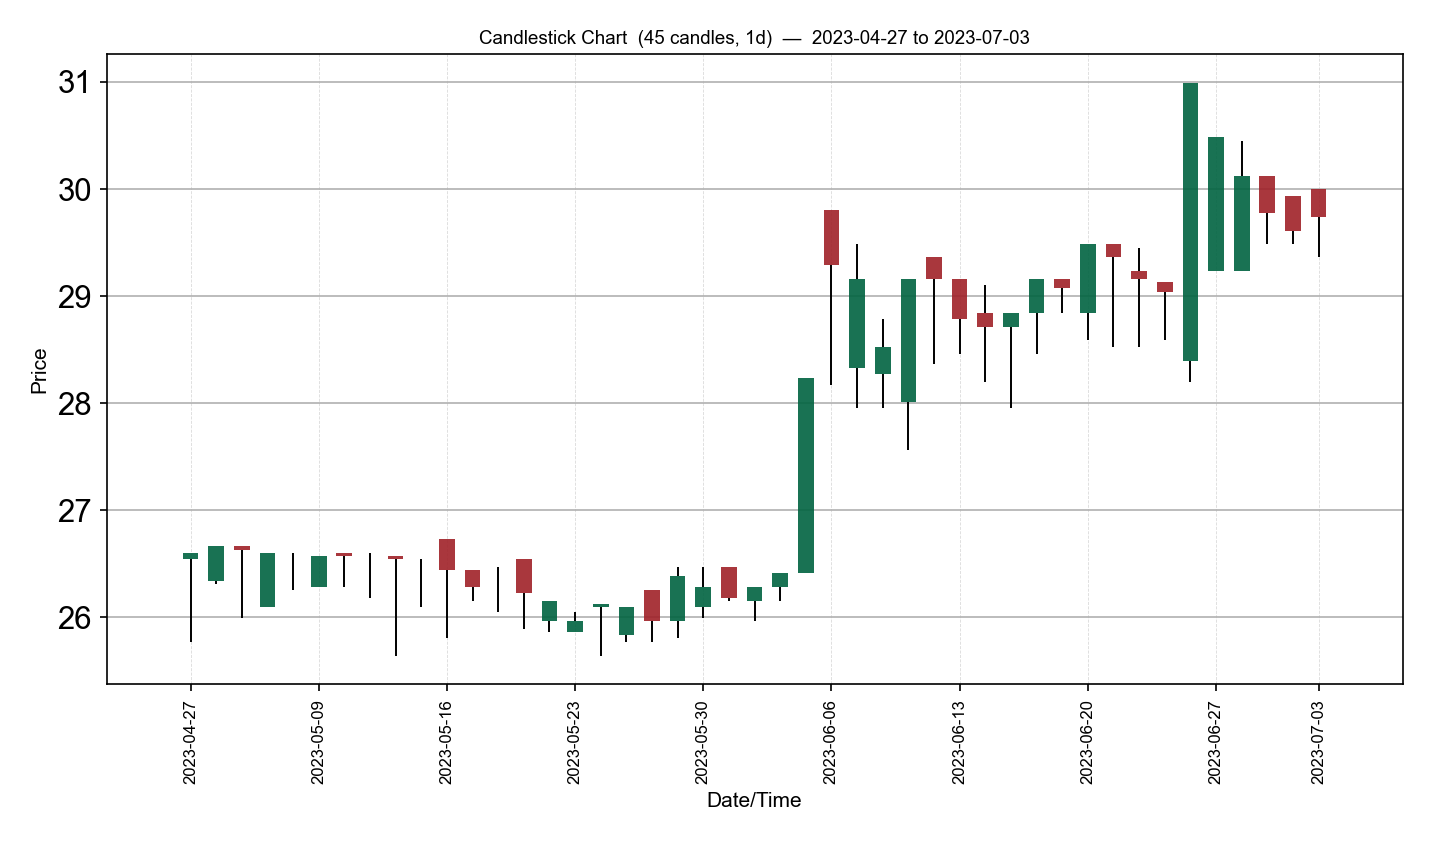
\includegraphics[width=0.90\textwidth]{figures/candlestick.png}\par\smallskip
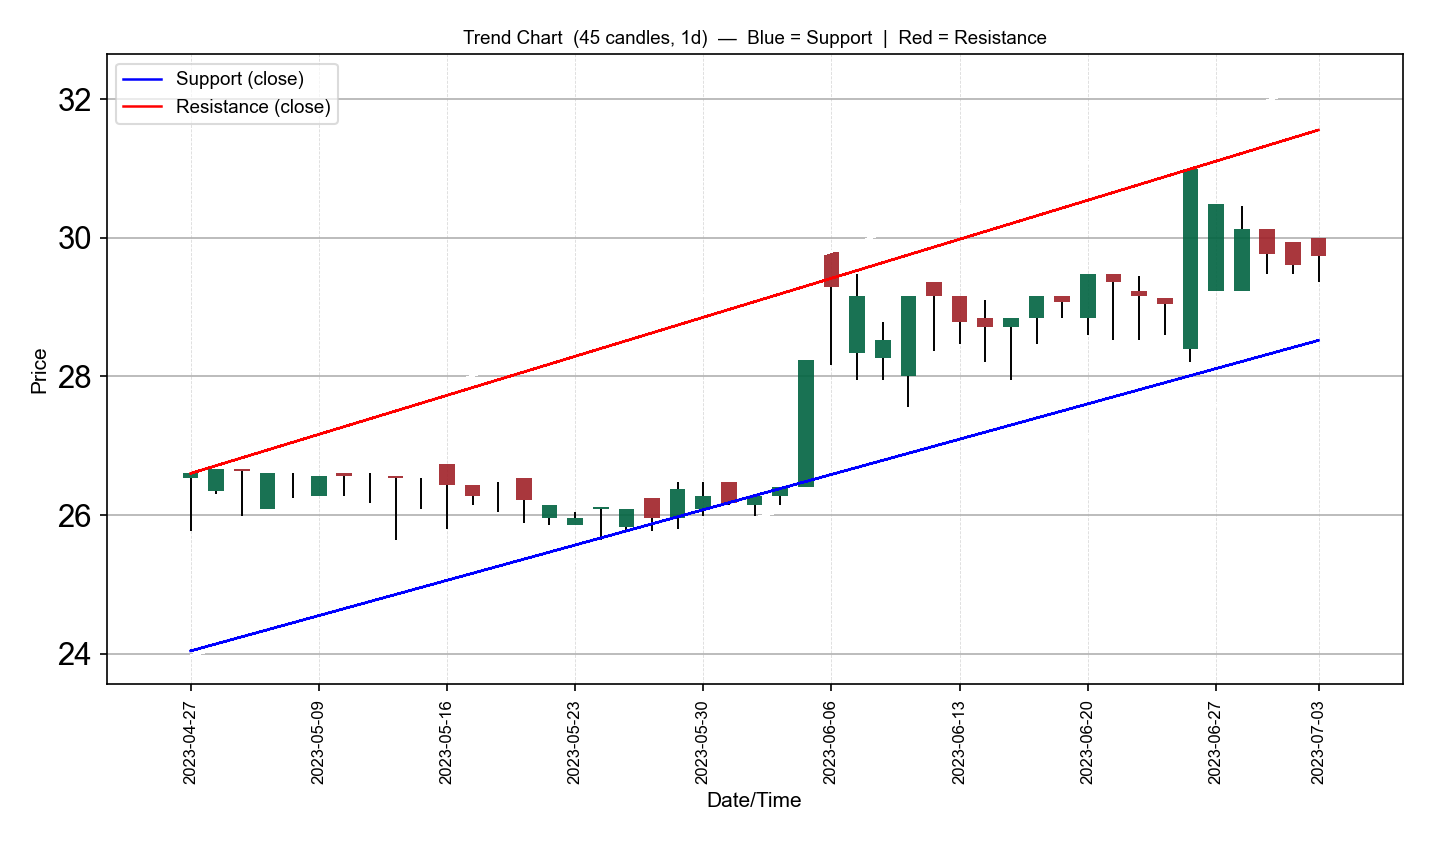
\includegraphics[width=0.90\textwidth]{figures/trendlines.png}
\caption{Candlestick and support--resistance inputs for CMG at the 3 July 2023 decision cutoff.}
\label{fig:charts}
\end{figure}

\subsection{Trend Agent}
Trend Agent receives a separate chart with fitted support/resistance lines. The inherited fitting utility starts with a least-squares close-price line, selects upper/lower deviation pivots, and optimizes a slope through each pivot under a non-crossing constraint. It implements both a close-only channel and a high/low channel, the latter using close-price regression to find pivots and high/low data for the bounds. These are numerical lines over the supplied window, not human-verified latent support levels.

For row position $u$, a fitted line has form $b+mu$. A support bound must remain below the corresponding price sequence within the implementation tolerance; resistance must remain above it. The local slope search reduces its step when the squared-deviation objective fails to improve or violates the constraint. The VLM then describes direction, levels, slope, price relative to support, forecast and confidence. Support is drawn blue and resistance red. A deterministic consistency check against simple price/trend summaries does not validate every reported level or coordinate.

Input checks match 204 chart images across 102 units byte for byte and pixel for pixel, and 240 recorded vision requests match their image caches and Vietnamese templates. The charts use blue support and red resistance lines, while the Vietnamese word \emph{xanh} is less colour-specific than the English term ``blue. Inherited high-frequency/K-line wording is used with daily bars, and the model's interpretation of these instructions is unverified.

\subsection{Decision Agent}
Decision receives condensed Indicator, Pattern and Trend reports plus enabled factor/sentiment sections. Reports are distilled and capped before prompt composition. The component study's observed successful Decision prompts are at most 4,187 characters, below the 6,500-character guard. Figure~\ref{fig:decision_agent} shows the extension dependencies, raw proposals, fallback and separate action policy.

\begin{figure}[htb]
\centering% Mũi tên giữa vai trò là dependency cùng repeat; policy tách raw/final.
\begin{tikzpicture}[>=Latex,
 box/.style={draw=blue!55!black,fill=blue!4,rounded corners,align=center,text width=4.8cm,minimum height=1.7cm,font=\footnotesize},
 wide/.style={box,text width=15.8cm},arr/.style={->,thick}]
\node[wide] (in) at (5.7,0) {\textbf{Shared reports $\rightarrow$ profile-specific prompt}\\Distil/cap; total prompt $<6{,}500$ characters; extension prior/context prefix $\le600$\\Retry and checkpoint interrupted requests. CASH requires a valid decision.};
\node[box] (native) at (0,-2.5) {\textbf{Our system}\\Native Decision prompt\\No extension dependency};
\node[box] (common) at (5.7,-2.5) {\textbf{Common Decision}\\Causal alpha / instructions\\Parent action for extensions};
\node[box] (prior) at (11.4,-2.5) {\textbf{Historical priors}\\Qualified historical context\\Support bypass $\rightarrow$ Common};
\draw[arr] (in.south)--++(0,-0.35)-|(native.north);
\draw[arr] (in.south)--(common.north);
\draw[arr] (common.east)--(prior.west);
\node[box] (fact) at (5.7,-5) {\textbf{Fact anchor}\\PIT facts + Common action\\Invalid assertions $\rightarrow$ Common};
\node[box] (mt) at (11.4,-5) {\textbf{BICL v5 revision}\\Common + anchor; tasks,\\student and teacher utility\\Ineligible context $\rightarrow$ anchor};
\draw[arr] (common.south)--(fact.north);
\draw[arr] (common.south east)--(mt.north west);
\draw[arr] (fact.east)--(mt.west);
\node[wide,fill=orange!7,minimum height=2cm] (policy) at (5.7,-7.9) {\textbf{Retain raw proposals; apply the specified external policy}\\Prior support bypass reuses Common; valid fact assertions select the anchor action.\\MT changes require valid assertions and $Q_{0.10}(\Delta U)>0$; otherwise retain the anchor.\\Persist final action, bypass/rejection reason and source proof for every role.};
\draw[arr] (native.south)--(native.south |- policy.north);
\draw[arr] (common.west)--(2.8,-2.5)--(2.8,-6.8)--(2.8,-6.8 |- policy.north);
\draw[arr] (prior.east)--(14.2,-2.5)--(14.2,-6.4)--(13,-6.4)--(13,-6.4 |- policy.north);
\draw[arr] (fact.south)--(fact.south |- policy.north);
\draw[arr] (mt.south)--(mt.south |- policy.north);
\node[wide,minimum height=1.35cm] (ledger) at (5.7,-10.3) {\textbf{Final action $\rightarrow$ outcome barrier $\rightarrow$ separate-account ledger}\\LONG: buy Open$(t+1)$, exit Close$(t+3)$, fee/slippage each leg; SHORT: CASH.\\Prompt priorities and model confidence are heuristics, not calibrated trading guarantees.};
\draw[arr] (policy)--(ledger);
\end{tikzpicture}

\caption{Decision dependencies, fallback rules and final-action policy.}
\label{fig:decision_agent}
\end{figure}

The instructions ask for trend/key-level assessment, recent-candle evidence, momentum confirmation and comparison with enabled factor/sentiment context. Price/chart evidence has priority, quantitative factors may challenge it, and sentiment has lower priority. These instructions describe an intended analysis sequence; they are not an independently observed internal reasoning trace or a guaranteed conflict-resolution algorithm.

The required output includes a binary LONG/SHORT forecast, forecast horizon, confidence, risk/reward field, evidence for/against and justification. Model confidence and risk/reward statements do not constitute calibrated uncertainty or executable price levels. In the long-only reference ledger, SHORT maps to CASH and LONG to the specified next-open/target-close cycle. The classifier's labels and account execution remain distinct.

Base retains the same upstream content and general instructions but removes both alpha and sentiment sections; those concepts may still appear in general instructions. Thus Full--Base changes a bundle and prompt length, not solely one numerical factor. Main/upstream prompts use compact factor text, whereas factorial A/AS/P deliver five explicit rows. The resulting representation difference remains part of the interpretation of the separate panels.

\paragraph{Historical-prior methods}
The \emph{Bayesian prior} (Bayesian in tables) retrieves up to three matured same-stock examples using regime and report-signal context. The \emph{conditional prior} (Conditional) adds Beta-based statistics matched on Trend/Pattern/Alpha/Indicator states, disjoint-background shrinkage and separate readiness checks for statistics and examples. The \emph{trend--pattern prior} (Trend--pattern) relaxes the statistics match to Trend/Pattern. The \emph{explicit-count prior} (Explicit counts) uses the conditional prior's support but explains counts, intervals and example identifiers more explicitly. Historical rates and plug-in intervals summarize the selected history; when no qualified prior is available, the method reuses Common's action for that repeat.

\paragraph{Fact anchor and MT-BICL}
Fact anchor receives a deterministic point-in-time fact packet, including MACD-versus-signal and Close-versus-SMA20 assertions, and the completed Common decision. Valid assertions select its proposed action without the numerical utility veto; invalid assertions select Common with a source proof. MT-BICL constructs numerical prior/target tasks conditioned on the factual bucket, retains a frozen student estimate and teacher-based utility summary, and requests a revision of that anchor only when context is eligible. The external policy in Eq.~\ref{eq:revision_utility} decides whether a changed proposal is accepted. Raw proposals, anchor actions, bypass and final actions are distinct saved fields, so final outcome differences cannot be assigned entirely to the LLM or student.

All extension prompts preserve report distillation/capping, require fewer than 6,500 characters and cap their prior/context prefix at 600 characters. The component-study maximum of 4,187 characters above is not an extension-run maximum. Exact prompt projections, readiness thresholds and request schemas are given in \ref{app:prompts} and~\ref{app:state_schema}; runtime resources and restore instructions are in \ref{app:software}.
\FloatBarrier
